\renewcommand{\theequation}{\theenumi}
\begin{enumerate}[label=\arabic*.,ref=\thesubsubsection.\theenumi]
\numberwithin{equation}{enumi}

\item In the given question,
\\
The sample size = Total Area of the rectangle=
\begin{align}
3x2=6 m^2
\end{align}
Favourable outcome = Area of Circle=
\begin{align}
\pi\brak{\frac{1}{2}}^2=\frac{\pi}{4} m^2 
\end{align}
Probabilty(P) of the dice landing in the circle=$\frac{\pi}{24}$
\\
$\therefore$ P = 0.131
\label{eq:prob}
\\
The python code for the figure \ref{fig:figure}
\begin{lstlisting}
prob/codes/prob1.py
\end{lstlisting}
shows the Bernouli distribution of data.
\begin{figure}[!ht]
\centering
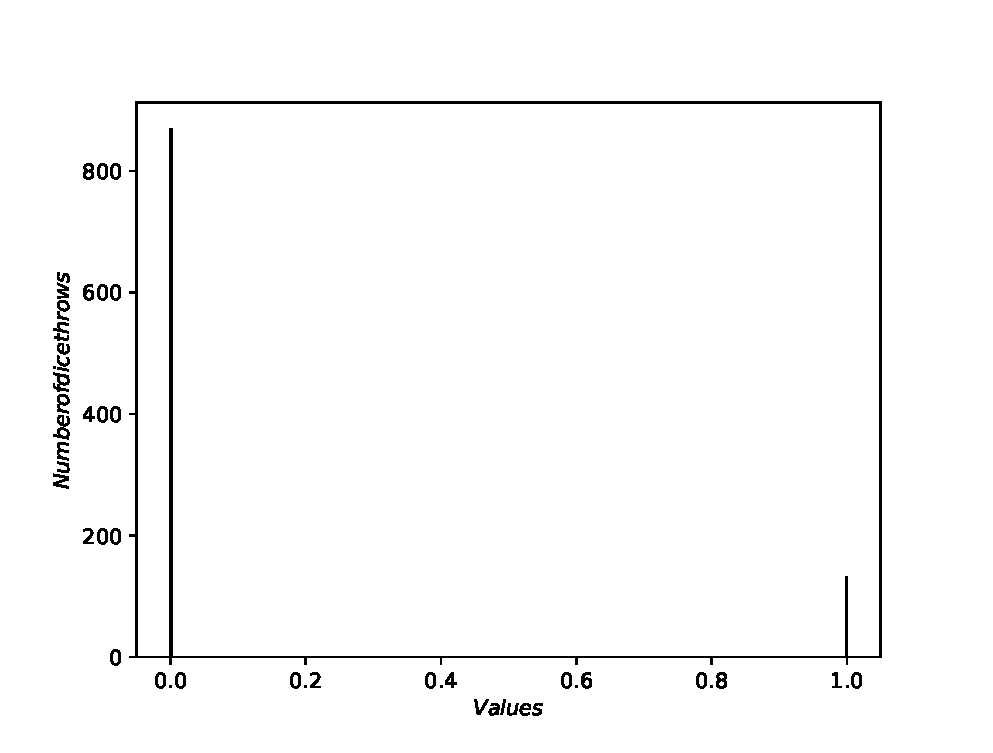
\includegraphics[width=\columnwidth]{./prob/figs/prob1.eps}
\caption{Bernoulli Distribution.}
\label{fig:figure}
\end{figure}
\\
The Bernoulli Distribution of data is given below
\\
Probability mass function(P(X))=$p^x\brak{1-p}^{1-x}$
\begin{align}
P(X=0)=1-p
\\
P(X=1)=p
\end{align}
where p=0.131 given by \ref{eq:prob}
\end{enumerate}